% !TeX document-id = {00a81f22-82a6-4b36-9e8d-aa862989e3df}
% !BIB TS-program = biber
\documentclass[twocolumn,10pt]{article}
\usepackage{graphicx} % images
\usepackage[T1]{fontenc} % Use 8-bit encoding that has 256 glyphs

\usepackage{microtype} % Slightly tweak font spacing for aesthetics

\usepackage[ngerman]{babel} % Language hyphenation and typographical rules

\usepackage[a4paper, left=2.5cm, right=2.5cm, top=2cm, bottom=2cm]{geometry} % Document margins
\usepackage[hang, small,labelfont=bf,up,textfont=it,up]{caption} % Custom captions under/above floats in tables or figures

\usepackage{lettrine} % The lettrine is the first enlarged letter at the beginning of the text

\usepackage{enumitem} % Customized lists
\setlist[itemize]{noitemsep} % Make itemize lists more compact

\usepackage{titlesec} % Allows customization of titles
\titleformat{\section}[block]{\large\scshape\centering}{\thesection.}{1em}{} % Change the look of the section titles
\titleformat{\subsection}[block]{\large}{\thesubsection.}{1em}{} % Change the look of the section titles

\usepackage{dirtytalk}
\usepackage{tabularx}
\usepackage{float}
\usepackage{acronym}
\usepackage[table, dvipsnames, svgnames]{xcolor}

\graphicspath{ {./images/} }

\author{Sven Hugi}
\title{IDAF - ChatGPT analysiert Songtexte}
\date{\today}

\makeatletter

\usepackage{fancyhdr} % Headers and footers
\pagestyle{fancy} % All pages have headers and footers

\fancyhead{} % Blank out the default header
\fancyfoot{} % Blank out the default footer
\fancyhead[L]{IDAF - ChatGPT analysiert Songtexte}
\fancyhead[R]{\today} % Custom header text
\fancyfoot[C]{\thepage} % Custom footer text
\fancyfoot[L]{Autor: Sven Hugi}

\usepackage{setspace}
%\singlespacing % spaceing 1.0
\onehalfspacing % spaceing, 1.5

\renewcommand{\arraystretch}{1}

%\pagestyle{fancy}
\captionsetup{font=footnotesize}


\usepackage[
style=numeric,
sorting=ynt,
backend=biber,
style=numeric
]{biblatex}

\addbibresource{idaf.bib}
\usepackage{wrapfig}

\usepackage{hyperref} % For hyperlinks in the PDF
% just all black
\hypersetup{
	colorlinks,
	citecolor=black,
	filecolor=black,
	linkcolor=black,
	urlcolor=blue
}
\renewcommand{\maketitle}{
	\begin{center}

		\vspace*{.125\textheight}
		{\Huge \textbf{\@title}\\}
		{\LARGE \textbf{\@author}\\}
		{\large \today\\}
		{\Large GIBB Berufsfachschule, Abteilung BMS\par\vspace*{1cm}}
		
\includegraphics[width=\linewidth]{title.png}
		\vfill
		\begin{center}
			\begin{tabularx}{.4\linewidth}{rl}
				\textbf{Art der Arbeit:}				& IDAF, Deutsch - Geschichte\\
				\textbf{Lehrpersonen:}					& Monika Michel, Ivo Knill\\
				\textbf{Abgabetermin:}					& 03.04.2023\\
				\textbf{Klasse:}						& Y2B	\\
				\textbf{Lizenz:}						& GNU FDL 1.3
			\end{tabularx}
		\end{center}
		
	\end{center}
}
\makeatother

\begin{document}
	\begin{titlepage}
		\maketitle
		\thispagestyle{empty}
	\end{titlepage}
	\onecolumn
	\pagestyle{fancy}
	\tableofcontents
	\clearpage
	\twocolumn
	
	\section{Einleitung}
		Diese Arbeit setzt sich mit dem AI-Language-Model ChatGPT\cite{ChatGPT} auseinander. Es wird überprüft, wie gut ChatGPT darin ist schwierige Texte zu analysieren. Dafür werden zwei Songs interpretiert. Der eine ist \say{Der Quell} von \say{Durbatuluk}, der andere ist \say{Angel Of Death} von \say{Slayer}. Es wird die volgende Frage versucht zu beantworten:\\
		\textbf{\say{Wie gut kann ChatGPT Songtexte von Metal Songs analysieren?}}
		\subsection{Übersicht}
		Im zuerst wird ChatGPT\cite{ChatGPT} im Grundsatz beschrieben. Dann folgt der Song \say{Der Quell} von \say{Durbatuluk}. Dabei wird zuerst der Musiker vorgestellt, dann wird der Songtext aufgezeigt, darauf folgt die analyse von ChatGPT und zum Schluss, was der Musiker selber zum Text sagt. \say{Der Quell} wurde für die Analyse gewählt, da der Text sehr komplex ist und die gesamte Meinung des Textes zwischen den Zeilen steht.\\
		Nach \say{Der Quell} wird der Song \say{Angel Of Death} von \say{Slayer} angeschaut. Der aufbau hier ist sehr ähnlich, zuerst wird die Band vorgestellt, dann der Songtext, darauf folgt die Analyse von ChatGPT und dann wird die Meinung der Band zum Song aufgegriffen. \say{Angel Of Death} wurde für die Analyse gewählt, da der Song sehr viel falsch verstanden wird, da er sich den Opfer des Holocaust widmet.
		\vfill
		\pagebreak
		\subsection{Persönliche Motivation}
		Als Informatiker bin ich an neuen Technologien sehr interessiert. ChatGPT ist dabei ein sehr spannendes Thema, welches in der Bildung immer wie mehr Relevanz gewinnt. Texte von ChatGPT können kaum von menschlichen Texten unterschieden werden und das AI-Language-Model ist sehr gut darin, prägnante, gut erklärende Texte über fast alle Themen zu schreiben.\\
		ChatGPT erleichtert unsere Arbeit enorm, da selbst technisch komplexe Probleme damit gelöst werden können. Wir haben es auf der Arbeit bereits hingekriegt, dass eine Aufgabe, welche auf einen Tag Aufwand geschätzt wurde, innert wenigen Minuten gelöst werden konnte.\\
		Zudem bin ich von Open Source Software begeistert. Open Source Software ist Software, von welcher man den Source Code bekommt und diesen analysieren kann und so nachvollziehen kann, wie die Software funktioniert. Dies ist viel besser für die User, da sie sich so sicher sein können, dass die Software auch das macht, was sie soll und nicht wie bei Software, die von Herstellern wie Microsoft kommt, der User nicht sicher sein kann, was die Software genau macht.\\
		Ich bin ausserdem Metalhead, sprich eine Person, die Metal hört, mit einer Kutte herumläuft, sich und andere Metalheads als \say{trve} / \say{trve kvlt} bezeichnet und die Musik als sehr wichtig erachtet.\\ 
		Metal hat anders als andere Musikrichtungen verhältnismässig sehr komplexe Texte (Wobei es auch Ausnahmen gibt).\\
		Ich bin vor allem in den extremeren Ecken des Metals interessiert, vor allem Black Metal, DSBM, Atmospheric Black Metal und Melodic Black Metal, aber auch Death und Thrash Metal, Folk Metal, Melodic Death Metal, Brutal Death metal usw.\\
		Ich bin auchunter anderem Fan des Oneman-Projects \say{Durbatuluk}, welches von Frank, besser bekannt als Farvann geführt wird. Dieser war so nett und hat sich bereitgestellt einen von seinen Songs genauer zu erläutern.\\
		Ich bin daran Motiviert, dass Leute sehen, dass Metal eine Musikrichtung ist, welche vielfältig ist, tiefgründige Texte hat und versucht aus etwas Negativem etwas Positives zu machen. Da ChatGPT an alltäglichen Daten Trainiert wurde, kann ich mir vorstellen, dass die AI gerade an Metal einige Probleme haben könnte. Es ist auf jeden Fall herausfordernd.
	\clearpage
	\section{Einführung in das Thema}
	ChatGPT\cite{ChatGPT} ist eine sehr weit entwickelte künstliche Intelligenz, welche sehr gute, menschenähnliche Texte generieren kann. Um die Stärke davon zu testen, werden Liedtexte von Metalsongs mit ChatGPT analysiert. Diese Analyse wird dann verglichen, mit dem, was Metalheads, bzw. der Songwriter dazu sagt. Durch die Komplexität dieser Songs ist es besonders schwierig, die Songs zu analysieren, weshalb davon relativ gut darauf geschlossen werden kann, wie gut ChatGPT im generellen ist und wo die Gefahren liegen.
	\subsection{ChatGPT}
	Wie funktioniert eigentlich ChatGPT\cite{ChatGPT}? Im folgenden Abschnitt wird dies versucht zu erklähren. Dabei wird auf den offiziellen Text von OpenAI\cite{openai_2022} gesetzt, jedoch auch persönliches Wissen über die Thematik verwendet. Um dies zu verstehen hilft es, wenn man die Mesh\cite{mesh} und Linked-List\cite{linkedlist} Datenstruktur versteht und sich den Code der Transformer-Models\cite{huggingface_2023} angeschaut hat.\\
	Es gilt zu beachten, dass dieser Text extrem grob zusammen gefasst ist, da man mit dem Thema locker eine Arbeit im Umfang von mehreren hundert Seiten schreiben kann.
	\subsubsection{Transformer}
	Ein Transformer-Model ist ein neuronales Netzwerk, welches Wörter miteinander verbindet. Ein Transformer-Model ist sehr günstig und effektiv zu trainieren, da die Daten nicht vorher ausgewertet werden müssen, sondern dies automatisiert beim Training passiert. Mit dieser Methode ist es einfach möglich, dass das Transformer-Model Wörter, wie es \say{versteht}. Wobei Verstehen das falsche Wort ist. Das Model versteht nichts, sondern kann nur Zusammenhänge aus Mustern erkennen. Dadurch kann das Transformer-Model jeweils das nächste Wort in einem Satz vorhersagen.
	\subsubsection{Reinforcement Learning from Human Feedback (RLHF)}
	Reinforcement Learning from Human Feedback ist eine Art, wie eine künstiliche Intelligenz anwendungsspezifisch trainiert werden kann, wenn bereits ein Transformer-Model existiert. Dabei wird (zumindest im Falle von ChatGPT) zuerst die Gewichtung ausgebaut, indem eine Prompt (Text-Input für den Transformer) gegeben wird und ein Output, welcher erwartet wird.\\
	In einem weiteren Schritt wird dies verfeinert, indem verschiedene Ausgaben generiert werden und diese nach der Qualität eingeordnet werden. Das fertig trainierte Model kann dan Texte schreiben, welche man fast nicht von einem menschlichen Text unterscheiden kann.
	\begin{figure}[H]
		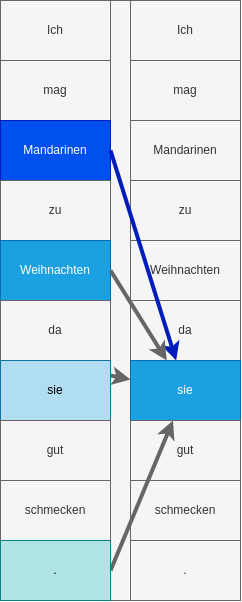
\includegraphics[width=.95\linewidth]{model}
		\caption{Transformer Model Beispiel}
	\end{figure}
	
	\pagebreak
	\section{Wie gut kann ChatGPT Songtexte analysieren?}
		Da Songtexte, gerade im Metal sehr komplex sind und viel Meinung dahinter steht, finde ich es sehr ausschlaggebend, wie gut eine AI diese Texte analysieren kann. Es ist äusserst komplex Zusammenhänge richtig zu interpretieren und die Meinung des Textes heruas zu finden. Viele Menschen haben nicht die analysischen Fähigkeiten, dies zu tun. Daher kann man davon ausgehen, dass eine AI sehr weit entwickelt sein muss, wenn sie dies kann. Die Songs wurden anhande ihrer Komplexität und Abstraktheit gewählt.
		\subsection{Durbatuluk - Der Quell}
			\say{Der Quell} ist ein Song von der EP \say{Aus anderen Augen}, die die Geschichte eines sterbenden Mannes im Krieg erzählt.\cite{Mail}\\
			\say{Der Quell} erzählt den Moment des Sterbens jenes Mannes. Der Song ist in sechs Verse aufgeteilt, einen Chorus gibt es nicht.
			\subsubsection{Frank / Farvann}
			\begin{wrapfigure}{L}{.5\linewidth}
				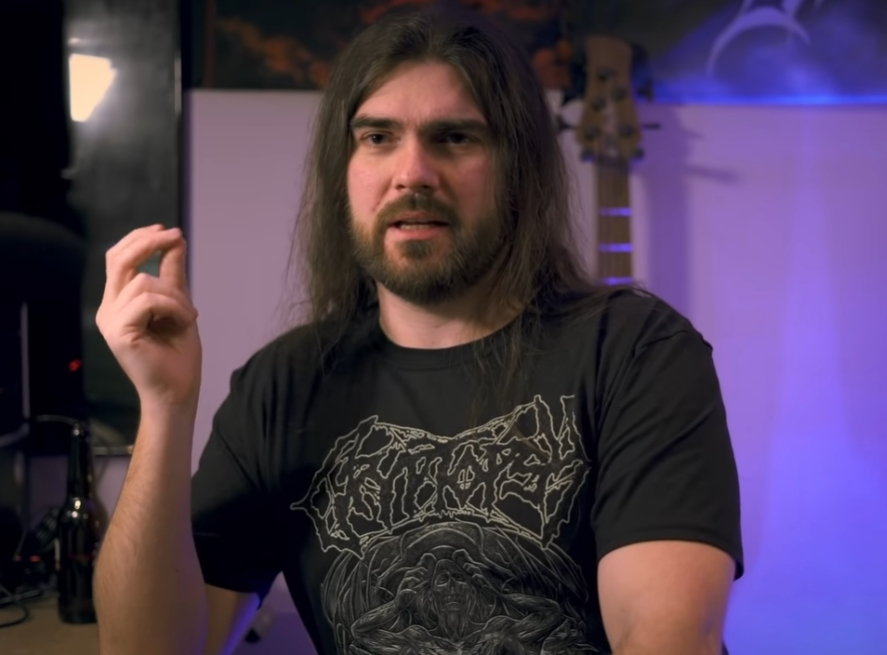
\includegraphics[width=\linewidth]{farvann.jpg}
				\caption{Farvann \cite{farvannImg}}
			\end{wrapfigure}
			Frank Busch, besser bekannt als Farvann\cite{farvann2023} ist ein Deutscher Musiker\cite{durbatulukbandcamp}, Youtuber\cite{youtubefarvann} und Softwareentwickler aus Heinsberg. Er wurde am 24. August 1989 geboren. Er ist Gitarist und Vokalist in der Grindcore-Band Document 6, sowie Gitarist, Bassist, Schlagzeuger und Sänger seines Oneman-Projects Durbatuluk.\\
			Auf Bandcamp\cite{durbatulukbandcamp} hat er die Folgenden EP, Alben und Demos veröffentlicht:
			\begin{itemize}
				\item Demo 2012
				\item The Very First Dream of Darkness (Demo 2014)
				\item Irrecoverably Lost
				\item Aus anderen Augen
				\item Erzähle, Baba Jaga
			\end{itemize}
		
			\pagebreak
			\subsubsection{Lyrics Der Quell}
			\begin{figure}[H]
				\centering
				
\includegraphics[width=.75\linewidth]{derQuell}
				\caption{Album Cover - Aus anderen Augen\cite{derQuellLyrics}}
			\end{figure}
		\begin{center}
			\textbf{Durbatuluk - Der Quell - Frank Busch\cite{derQuellLyrics}}\\
			\textit{Heller ist mein Licht}\\
			\textit{Fern bin ich von euch}\\
			\textit{Fremd bin ich geworden}\\
			\textit{Unten, weit oben?}
\vspace{11pt}\\
			\textit{Stets seid ihr präsent}\\
			\textit{Alle um mich vereint}\\
			\textit{Grauen, Heil und Wohlgemach}\\
			\textit{Alles ist mein Sein}
\vspace{11pt}\\
			\textit{Spreche ich von Versagen}\\
			\textit{Ihr versteht, ihr versteht}\\
			\textit{Spreche ich von Verlangen}\\
			\textit{Ihr versteht, ihr versteht}
\vspace{11pt}\\			
			\textit{Sprechen wir von Verstand}\\
			\textit{Hört ihr zu, ihr hört zu}\\
			\textit{Spreche ich durch euch}\\
			\textit{Warum hört ihr euch nicht zu?}
\vspace{11pt}\\
			\textit{Meine Welt ist ungewiss}\\
			\textit{Und Welten gibt es doch zuhauf}\\
			\textit{Dem Morgen bin ich entflohen}\\
			\textit{Doch das Gestern bleibt mein Stein}
\vspace{11pt}\\
			\textit{Durch den Kosmos rinnt mein Ich}\\
			\textit{Ihr versteht, ihr versteht nicht}\\
			\textit{Eine weitere Quelle fliesst}\\
			\textit{Es ist eine von vielen}			
		\end{center}
			\clearpage
			\subsubsection{Analyse ChatGPT}
			ChatGPT\cite{ChatGPT} hat die folgende Antwort geliefert, als sie gefragt wurde, den Song \say{Der Quell} von \say{Durbatuluk} so detailiert, wie möglich zu analysieren und zwischen den Zeilen zu lesen. Um eine möglichst gute Interpretation zu erhalten, wurde in Englisch gefragt.\vspace{11pt}\\
			\textit{The song \say{Der Quell} by Durbatuluk is a complex and thought-provoking piece of black metal music. The lyrics are written in a poetic and metaphorical style, and they touch on themes of isolation, identity, and the search for meaning in an uncertain world.}\vspace{11pt}\\
			\textit{The first verse begins with the line \say{Heller ist mein Licht} (\say{Brighter is my light}), which could be interpreted as a statement of confidence or clarity. However, the following lines suggest a sense of distance and detachment from others: \say{Fern bin ich von euch / Fremd bin ich geworden / Unten, weit oben?} (\say{Far am I from you / Alien I have become / Below, far above?}). These lines could be read as an expression of alienation from society or from one's own sense of self.}\vspace{11pt}\\
			\textit{The second verse presents a seemingly contradictory image of being \say{um mich vereint} (\say{surrounded by all of you}) while still feeling a sense of detachment or disconnection. The line \say{Grauen, Heil und Wohlgemach / Alles ist mein Sein} (\say{Horror, salvation and comfort / All is my being}) could be interpreted as an assertion of the speaker's power or dominance over these experiences or emotions.}\vspace{11pt}\\
			\textit{The third verse delves into the difficulty of communication and the limitations of language. The speaker notes that when they speak of failure, desire, or reason, others may understand but not truly listen. The line \say{Spreche ich durch euch / Warum hört ihr euch nicht zu?} (\say{I speak through you / Why do you not listen to yourselves?}) suggests that perhaps the speaker's own voice is not being heard or understood, or that others are not truly hearing themselves either.}\vspace{11pt}\\
			\textit{The fourth verse presents a sense of uncertainty and impermanence, with the speaker's world being \say{ungewiss} (\say{uncertain}) and there being countless other worlds out there. The lines \say{Dem Morgen bin ich entflohen / Doch das Gestern bleibt mein Stein} (\say{I have escaped the morning / But yesterday remains my stone}) suggest a desire to escape the present and the future, but an inability to fully let go of the past.}\vspace{11pt}\\
			\textit{The final lines of the song are perhaps the most enigmatic: \say{Durch den Kosmos rinnt mein Ich / Ihr versteht, ihr versteht nicht / Eine weitere Quelle fliesst / Es ist eine von vielen} (\say{My self runs through the cosmos / You understand, you do not understand / Another source flows / It is one of many}). These lines could be read as a meditation on the nature of identity and consciousness, with the self being seen as a fluid and constantly changing entity that is just one of many in the universe.}\vspace{11pt}\\
			\textit{Overall, \say{Der Quell} is a dense and layered work of art that rewards close reading and interpretation. The lyrics touch on universal themes of identity, communication, and the search for meaning, while also incorporating esoteric and philosophical ideas.}\vspace{11pt}\\
			Zusammengefasst und auf Deutsch übersetzt ergiebt das in etwa:\\
			\say{Der Quell} von Durbatuluk ist ein komplexes und tiefgründiges Black Metal Lied, das poetische und metaphorische Texte über Isolation, Identität und die Suche nach Bedeutung in einer unsicheren Welt enthält. Die Texte spiegeln Gefühle von Entfremdung, Macht und Unsicherheit wider.\\
			Der Song startet mit einem erklähren von Selbstsicherheit und Abstand zu Anderen, so wie die Verfremdung zur Gesellschaft und zu sich.\\
			Der zweite Vers spricht davon von sich selber umgeben zu sein.\\
			Der Drite spricht von schwieriger Kommunikation.\\
			Der Vierte spricht von einer unklaren Welt und dem Willen der Gegenwart und der Zukunft zu entfliehen aber die Vergangenheit nicht loslassen zu können.\\
			Die letzten Zeilen sprechen davon, eine Meditation aus Identität und Bewustsein zu sein und sich selber als flüssiges, sich immer änderndes Ding zu sein, das es mehrfach im Universum gibt.\\
			Dabei ist zu beachten, dass dieser Text von mir übersetzt und zusammengefasst wurde und womöglich nicht genau so von ChatGPT\cite{ChatGPT} angedacht war, weshalb der englische Originaltext für Analysen verwendet wird.
			\pagebreak
			\subsubsection{Worte von Frank}
			Ich habe die Interpretation von ChatGPT an Frank gesendet, dieser hat dann in einem Mail\cite{Mail} dazu folgendes gemeint:\\
			\textit{[...] das was ChatGPT da interpretiert völliger Blödsinn ist.}\\
			\textit{Ganz grob gesagt beschreibt die ganze EP \say{Aus Anderen Augen} das Sterben eines Mannes im Krieg.}\\
			\textit{Im ersten Song \say{Hingabe} wird die Geschichte aus Sicht des Kameraden erzählt, der vom Tod seines Gefährten schreibt/berichtet bzw. erlebt.}\\
			\textit{\say{Der Quell} erzählt vom Moment des Sterbens eben jenes Gefährten:}
			\begin{center}
				\say{\textit{Heller ist mein Licht}\\
					\textit{Fern bin ich von euch}\\
					\textit{Fremd bin ich geworden}\\
					\textit{Unten, weit oben?}}
			\end{center}
			\textit{Er realisiert gerade erst, dass er tot ist. Er tritt in das bekannte \say{grelle Licht} von dem so viele Nahtoderfahrungen berichten. Fremd (ein Geist?) ist er geworden, noch nicht dazu in der Lage, den Ort zu beschreiben, an dem er sich nun befindet (Unten, weit oben?)}
			\begin{center}
				\say{\textit{Stets seid ihr präsent}\\
				\textit{Alle um mich vereint}\\
				\textit{Grauen, Heil und Wohlgemach}\\
				\textit{Alles ist mein Sein}}
			\end{center}
			\textit{Soll beschreiben, wie der Tote nun \say{Zeit} erfährt. Hängt mit meiner ganz persönlichen Vorstellung vom Konzept der Zeit zusammen, weil ich glaube, dass Zeit, genau wie der Raum, eine Dimension ist, durch die man \say{wandern kann} (um es dreidimensional auszudrücken). Da er nun tot ist, ist er nicht mehr an das lineare Zeitverständnis gebunden, das sich unser menschliches Gehirn zusammenbastelt. Er fühlt sich nun vollständig als Teil des Ganzen. Was auch immer \say{das Ganze} ist, bleibt natürlich verborgen. Um das zu beschreiben reichen meine textlichen Fähigkeiten einfach nicht aus. Und als alter David Lynch Fan bin ich immer ein Freund davon, niemals alles aufzudecken. Win-Win-Situation an dieser Stelle aus Songschreiber-Sicht also.}
			\begin{center}
				\say{\textit{Spreche ich von Versagen}\\
				\textit{Ihr versteht, ihr versteht}\\
				\textit{Spreche ich von Verlangen}\\
				\textit{Ihr versteht, ihr versteht}\vspace{11pt}\\
				\textit{Sprechen wir von Verstand}\\
				\textit{Hört ihr zu, ihr hört zu}\\
				\textit{Spreche ich durch euch}\\
				\textit{Warum hört ihr euch nicht zu?}}
			\end{center}
			\textit{Das soll eigentlich nur beschreiben, dass die Lebenden nicht sehen / erleben können, was er sieht, obwohl sie doch bereits in dieser grossen allumfassenden Welt leben und, genau wie er, erfahren. Er spricht also durch das, was auch immer er nun ist, mit den Menschen}
			\begin{center}
				\say{\textit{Meine Welt ist ungewiss}\\
				\textit{Und Welten gibt es doch zuhauf}\\
				\textit{Dem Morgen bin ich entflohen}\\
				\textit{Doch das Gestern bleibt mein Stein}}
			\end{center}
			\textit{Hier versucht er, mit irdischen Worten wie \say{Morgen}, \say{Gestern} oder dem \say{(Grab)-Stein} zu beschreiben was er erlebt, scheitert jedoch, da Worte an diesem Punkt nicht ausreichen.}
			\begin{center}
				\say{\textit{Durch den Kosmos rinnt meint Ich}\\
					\textit{Ihr versteht, ihr versteht nicht}\\
					\textit{Eine weitere Quelle fliesst}\\
					\textit{Es ist eine von vielen}}
			\end{center}
			\textit{Das hier geht eigentlich schon eher in Richtung Quantenmechanik oder Multiversum-Theorie (\say{eine weitere Quelle fliesst}).}\\
			\textit{Wenn die Urknall-Theorie stimmt, dann war \textbf{ALLES} ursprünglich mal auf einen einzigen Ort konzentriert. Jeder Berg, jedes Meer, jede Sonne, jede Galaxie und jedes Lächeln und Weinen war vor 14 Milliarden Jahren schon da und wird seitdem wie durch einen Projektor, den wir \say{Zeit} nennen, auf eine Leinwand projiziert. Der Urknall. Der Quell.}\\
			\textit{Das erlebt dieser sterbende Soldat in diesem Augenblick und versucht es in Worte zu fassen.}\\
			\textit{\say{Der Quell} handelt von den allerersten Momenten, die der Sterbende erfährt. Als Kontrast zu den allerletzten Momenten, die sein Kamerad (in \say{Hingabe}) mit ihm erlebte.}
		\clearpage
		\subsection{Slayer - Angel Of Death}
			\say{Angel Of Death} ist der erste Song auf dem Album \say{Regin in Blood} aus 1986 von der amerikanischen Thrash Metal Band Slayer. Der Song wurde von Jeff Hanneman geschrieben und handelt über den Nazi Doktor Josef Mengele, welcher im zweiten Weltkrieg im KZ-Auschwitz grausame Experimente an Insassen vorgenommen hat.\\
			Der Song ist wie für Slayer typisch sehr brutal und beschreibend. Der Song beschreibt sehr grafisch die grausamen experimente von Mengele. Empfindliche Personen sollten daher die Lyrics in Unterkapitel \autoref{laod} nicht lesen.
			\subsubsection{Slayer}
			\begin{figure}[H]
				
\includegraphics[width=\linewidth]{slayer-2016}
				\caption{Slayer - 2016 - Overdrive\cite{overdrive_2018}}
			\end{figure}
			Slayer ist eine Thrash-Metalband aus Huntington Park, California, USA, sie wurden 1981 gegründet und gehört zu den Big 4 of Thrash Metal (Metallica, Anthrax, Megadeth und Slayer). Sie ist dabei bekannt dafür den brutalen (brvtal) aggresivsten und ungezähmtesten Sound. Slayer hat mit ihrem besonders schnellen, harten und dunklen Sound die Thrash-Metal-Geschichte massgeblich geformt und vile Bands beeinflusst. Slayer selber wurde von Bands, wie Iron Maiden, Judas Priest, Motörhead, aber auch einigen Punk Bands beeinflusst.\\
			Slayer singt vor allem über Krieg, Leiden, Serienmörder, Genozid, Folter, Rassismus, Faschismus und Satanismus, wobei Tom Araya aber ein gläubiger Katholik ist.\\
			Das originale Layout bestand aus Tom Araya als Sänger und Bassist, Jeff Hanneman als Gitarist, Dave Lombardo als Schlagzeuger und Kerry King auch as Gitarist.\\
			Später kammen noch dazu: Paul Bostaph als Schlagzeuger, Gary Holt als Ersatz von Jeff, nach dessen Tod, Tony Scalione als Schlagzeuger und Jon Datte auch als Schlagzeuger. \cite{slayer.net}\\
			Der Band wurde mehrfach Satanismus und antireligiöses Verhalten vorgeworfen. Besonders in der USA gab es Klagen gegen die Band\cite{nme_2001}, jedoch wurden alle abgewiesen, da sie keinen Sinn ergeben haben, bzw. Zusammenhänge fehlten. Dies ist besonders ironisch, wenn man bedenkt, wie religiös der Frontmann Tom Araya ist und was er zu Slayer und Religion zusagen hat.\\
			Dies führte später zu der Aussage: \say{Jesus listens to Slayer}, welche vor allem in der Meme-Kultur Beliebtheit gefunden hat.
			\begin{figure}[H]
				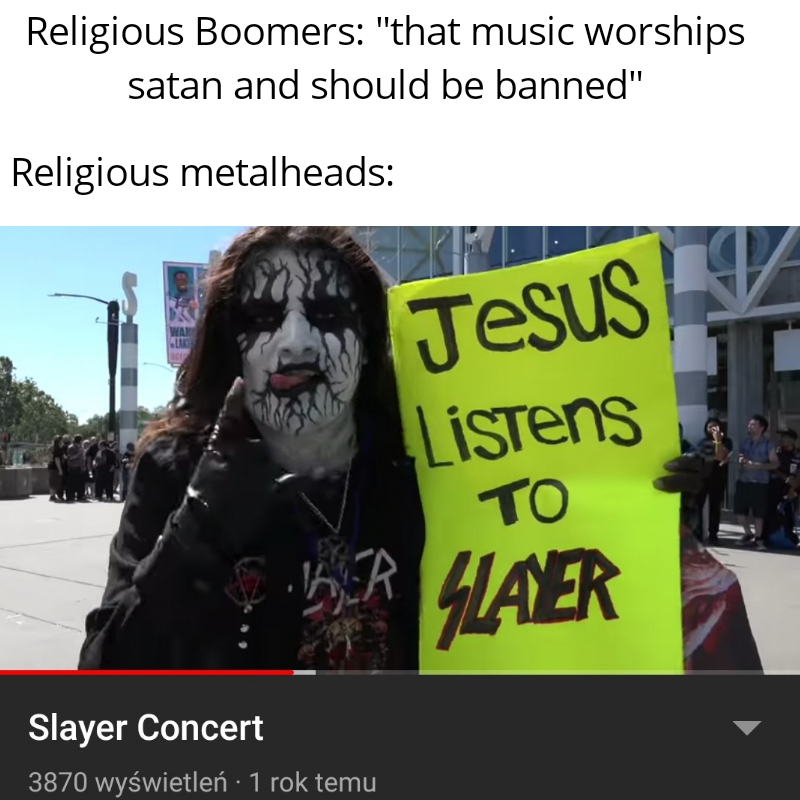
\includegraphics[width=\linewidth]{jesus}
				\caption{Meme - metalpoleguy16\cite{jesus}}
			\end{figure}
			\clearpage
			\subsubsection{Lyrics Angel Of Death}\label{laod}
			\begin{figure}[H]
				\centering
\includegraphics[width=\linewidth]{ReignInBlood.jpg}
				\caption{Album Cover - Reign In Blood\cite{aodLyrics}}
			\end{figure}
			\begin{center}
			\textbf{Slayer - Angel Of Death - Jeff Hanneman\cite{aodLyrics}}\\
			\textbf{[Verse 1]}\\
			\textit{Auschwitz, the meaning of pain}\\
			\textit{The way that I want you to die}\\
			\textit{Slow death, immense decay}\\
			\textit{Showers that cleanse you of your life}\\
			\textit{Forced in; like cattle, you run}\\
			\textit{Stripped of your life's worth}\\
			\textit{Human mice for the Angel Of Death}\\
			\textit{Four hundred thousand more to die}
			\vspace{10pt}\\
			\textbf{[Chorus]}\\
			\textit{Angel Of Death}\\
			\textit{Monarch to the kingdom of the dead}
			\vspace{10pt}\\
			\textbf{[Verse 2]}\\
			\textit{Sadistic, surgeon of demise}\\
			\textit{Sadist of the noblest blood}\\
			\textit{Destroying without mercy}\\
			\textit{To benefit the Aryan race}\\
			\textit{Surgery with no anesthesia}\\
			\textit{Feel the knife pierce you intensely}\\
			\textit{Inferior, no use to mankind}\\
			\textit{Strapped down, screaming out to die}
			\vspace{10pt}\\
			\textbf{[Chorus]}\\
			\textit{Angel Of Death}\\
			\textit{Monarch to the kingdom of the dead}\\
			\textit{Infamous butcher}\\
			\textit{Angel Of Death}
			\vspace{10pt}\\
			\textbf{[Verse 3]}\\
			\textit{Pumped with fluid inside your brain}\\
			\textit{Pressure in your skull begins}\\
			\textit{Pushing through your eyes}\\
			\textit{Burning flesh drips away}\\
			\textit{Test of heat burns your skin}\\
			\textit{Your mind starts to boil}\\
			\textit{Frigid cold cracks your limbs}\\
			\textit{How long can you last}\\
			\textit{In this frozen-water burial?}\\
			\textit{Sewn together, joining heads}\\
			\textit{Just a matter of time}\\
			\textit{Till you rip yourselves apart}
			\vspace{10pt}\\
			\textbf{[Bridge]}\\
			\textit{Millions laid out in their}\\
			\textit{Crowded tombs}\\
			\textit{Sickening ways to achieve}\\
			\textit{The Holocaust}
			\vspace{10pt}\\
			\textbf{[Verse 4]}\\
			\textit{Seas of blood bury life}\\
			\textit{Smell your death as it burns}\\
			\textit{Deep inside of you}\\
			\textit{Abacinate, eyes that bleed}\\
			\textit{Praying for the end of}\\
			\textit{Your wide-awake nightmare}\\
			\textit{Wings of pain reach out for you}\\
			\textit{His face of death staring down}\\
			\textit{Your blood's running cold}\\
			\textit{Injecting cells, dying eyes}\\
			\textit{Feeding on the screams of}\\
			\textit{The mutants he's creating}
			\vspace{10pt}\\
			\textbf{[Bridge]}\\
			\textit{Pathetic, harmless victims}\\
			\textit{Left to die}\\
			\textit{Rancid Angel Of Death}\\
			\textit{Flying free}
			\vspace{10pt}\\
			\textbf{[Chorus]}\\
			\textit{Angel Of Death}\\
			\textit{Monarch to the kingdom of the dead}\\
			\textit{Infamous butcher}\\
			\textit{Angel Of Death}\\
			\textit{Angel Of Death}		
			\end{center}
			\clearpage
			\subsubsection{Analyse ChatGPT}
			Ich habe ChatGPT\cite{ChatGPT} folgendes gefragt: \say{analyze the lyrics and meaning of the song Angel Of Death from slayer in detail}\vspace{10pt}\\
			\textit{\say{Angel Of Death} is a controversial song by American thrash metal band Slayer, released in 1986. The lyrics are written from the perspective of Josef Mengele, a notorious Nazi doctor who conducted horrific medical experiments on prisoners during the Holocaust. The song has been the subject of much debate and criticism due to its graphic and disturbing content.}\\
			\textit{The lyrics describe in detail the atrocities committed by Mengele, including his medical experiments on twins and his involvement in the selection process at Auschwitz. The song's chorus, \say{Angel Of Death, Monarch to the kingdom of the dead,} suggests that Mengele was a symbol of death and destruction.}\\
			\textit{The opening lines of the song, \say{Auschwitz, the meaning of pain / The way that I want you to die,} set the tone for the rest of the lyrics. The song also contains references to the notorious SS officer Rudolf Höss and the infamous \say{Final Solution} of the Nazi regime. The lyrics are graphic and violent, and describe the horrors of the Holocaust in detail.}\\
			\textit{The song has been widely criticized for its subject matter and graphic content, with some accusing Slayer of promoting Nazi ideology or trivializing the Holocaust. However, the band has defended the song as a critique of Mengele and the horrors he committed, and have emphasized that they do not condone or support Nazi ideology in any way.}\\
			\textit{Overall, \say{Angel Of Death} is a highly controversial song that has sparked intense debate and criticism. While the song's graphic lyrics and subject matter are undeniably disturbing, some argue that it serves as a powerful critique of the atrocities committed during the Holocaust, while others argue that it is inappropriate to use such a subject matter for entertainment purposes.}\\
			Zusammengefasst und übersetzt ergibt das etwa:\\
			\say{Angel Of Death} ist ein umstritener Slayer Song von 1986 aus der Perspektive von Josef Mengele, einem berüchtigten Nazi-Arzt, der während des Holocausts grausame medizinische Experimente an Häftlingen durchführte. Der Song beschreiben die Taten von Mengele und die Schrecken des Holocausts. Während einige argumentieren, dass es als mächtige Kritik an den Holocausts dient, kritisieren andere es dafür, dass es den Holocaust trivialisiere oder sogar Nazi-Ideologie fördere.
			\subsubsection{Worte von Slayer}
			Der folgende Text stammt aus einem Interview von Knac.com\cite{slayerInterview} und wurde gekürtzt und übersetzt.\\
			Hanneman meinte: \say{In den Anfängen war einfach nichts zutun. Es gab kein Tourbus, wir sind mit Autos umher gefahren, es gab einfach nichts zu tun, also habe ich Bücher über den zweiten Weltkrieg gekauft und gelesen.}\\
			Auf die Frage, ob dies seinen Schreiben beeinflussen würde, antwortete Hanneman: \say{Ja. Bevor ich Angel Of Death geschrieben habe habe ich ein paar Bücher über Mengel gelesen, da er verdammt krank ist. Das war, wie der Song zustande kamm.}\\
			Er wurde darauf gefragt, ob es eine grosse Missinterpretation sei, dass leute Slayer als Nazis, Satanisten und Rassisten einschätzen, da sie damit gehen \say{Oh mein Gott! Angel Of Death -- das ist so pro-Nazi!} Hanneman antwortete darauf: \say{Ich weiss, warum Leute das so missinterpretieren. Es ist einfach eine Kurzschlussreaktion. Wenn sie den Text lesen und dann ist nichts drin, wo ich sage, dass er ein schlechter Mann ist. Ist das aber nicht offensichtlich?! Ich sollte das nicht erklähren müssen.}\\
			Er wird dann gefragt, ob es eines der taboo Themen sei, wo Leute direkt die Falscheinschätzung machen, dass jemand Nazi sei, nur weil er es anspricht. Worauf Hanneman sarkatisch antwortet: \say{Genau, nur weil wir nicht sagen, dass es sehr schlecht ist.}\\
			Der Interviewer sagt dann sarkastisch: \say{Also hören wir nicht was sie sagen oder was im Text steht und machen einfach jetzt Annahmen.}\\
			Hanneman bestätigt dies mit: \say{Genau, es ist eine Kurzschlussreaktion ala: Huh?, Oh mein Gott!!!}
			\begin{figure}[H]
				\centering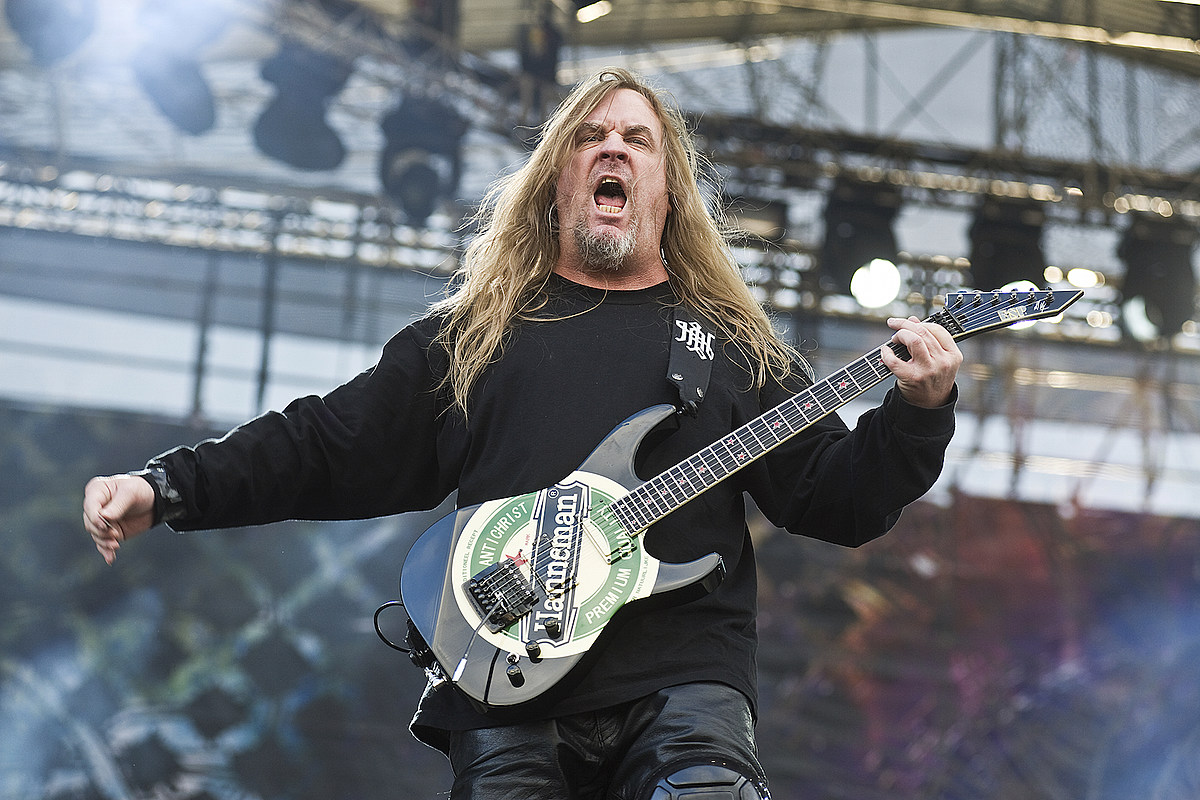
\includegraphics[width=.97\linewidth]{jeff.jpeg}
				\caption{Jeff Hanneman - Jon Widerhorn\cite{jonwiederhorn_2022}}
			\end{figure}
			
			\clearpage
			\subsubsection{Interpretation von Metalheads}
			Durch eine Befragung auf dem Farvann-Discord-Server sind einige Meinungen von anderen Metalheads zusammen gekommen.\\
			lekille screibt:
			\begin{center}
			\textit{When it comes to slayer's angel of death, it does extremely little to make themselves out as nazis. Considering the rampant satanic themes in slayer and metal generally, to use a nazi mass murder and torturer as topic for a song should be expected. In no way does the song glorify or give admiration, simply takes the horrible things mengeles did and made a song out of it}	
			\end{center}
			Auf Deutsch: \say{Wenn es um Slayers Angel of Death geht, tut es extrem wenig, um sie als Nazis darzustellen. In Anbetracht der weit verbreiteten satanischen Themen in Slayer und im Metal im Allgemeinen, sollte man erwarten, dass ein Nazi-Massenmörder und Folterknecht als Thema für einen Song verwendet wird. Der Song verherrlicht oder bewundert in keiner Weise die schrecklichen Dinge, die Mengeles getan hat, und macht daraus einen Song.}\\
			Jason.jpeg schreibt:
			\begin{center}
				\textit{Angel of Death geht um den NS Offizier Josef Mengele, der mehrere tausend Menschen in Experementen getötet hat (darunter zählt Köpfe zusammennähen, Zellen in Augen reinspritzen etc)}\\
				\textit{Das Lied selber hat keine verteidigende Meinung, aber auch keine offensive, weshalb es aus dem Grund als Naziverherrlichung dargestellt wurde.}
			\end{center}
			Meine Meinung:
			\begin{center}
				\textit{Slayer ist eine Band, die über Geschichte singt. Das macht sie doch nicht zu Nazis. Gerade wenn man bedenkt, dass sie Thrash-Metal produzieren. Da geht es um Provokation, um das Kritisieren und um das Zeigen von Problemen.}\\
				\textit{Nur weil ein paar Leute nicht lesen können oder die Musik nicht verstehen, sollten sie die Band nicht als Nazis abstempeln.}\\
				\textit{Ich meine du beleidigst dein Geschichtslehrer ja auch nicht als Nazi, da er zeigt, was für Experimente Mengele durchgeführt hat und dabei nicht sagt, dass er ein schlechter Mensch war.}\\
				\textit{Leute, die eine Band nicht verstehen und sich auch keine Mühe geben, sie zu verstehen sollten ihr Maul halten und nicht falsche Informationen über die Band verbreiten.}\\
				\textit{Du kannst jeden Metalhead fragen, was er über Slayer denkt und keiner wird dir sagen, dass sie Nazis sind.}
			\end{center}
		\subsubsection{Analyse der Analyse von ChatGPT}
		ChatGPT ist in der Lage, den Song richtig zu datieren und erkennt die Band. ChatGPT behaupted, dass der Song aus der Perspektive von Mengele geschrieben würde, obwohl der Song am Anfang den Text \say{The way that I want you to die} beinhaltet, wird Mengele später als \say{Infamous butcher} referenziert. Jeff Hanneman hat  die Perspektive nie verraten. Jedoch ist der ganze Song wie eine Dokumentation geschrieben, weshalb zu bezweifeln ist, ob die Perspektive aus Sicht von Mengele ist.\\
		Das Mengele von Slayer als Symbol des Todes dargestellt wird ist richtig und auch Typisch für Slayer.\\
		Die Referenz zu Höss ist jedoch nicht, bzw. nicht direkt gegeben. Jedoch wird über \say{Destroying without mercy to benefit the Aryan race} gesungen (Zerstören ohne Erbarmen um der arischen Rasse zu helfen) was die Vernichtung der Juden im zweiten Weltkrieg, Hittlers \say{Endlösung} anspricht.\\
		Es ist richtig, dass der Text sehr Grafisch und Brutal ist, dies ist typisch für Slayer. Auch die Beschreibung des Holocaust im Detail ist richtig.\\
		Dass der Song kritisiert wird ist ebenfalls richtig.\\
		ChatGPT sagt, dass der Text ohne Zweifel verstörend sind, aber es die einige sagen, dass es Kritik am Holocaust sei, während andere sagen, dass es unangebracht sei über dieses Thema zu schreiben. Was alles auch richtig ist.\\
		Die Analyse von ChatGPT ist bis auf wenige Ausnahmen wirklich gut und nicht wirklich von einer menschlichen Analyse zu unterschieden. 
			
		\vfill
		\clearpage
	\section{Fazit}
	Durch dieses Experiment kann man gut aufzeigen, dass ChatGPT\cite{ChatGPT} eben doch nicht immer gute Texte leifern kann. Die Interpretationen sind zwar glaubhaft, aber gerade im Fall von \say{Der Quell} alles andere als Richtig.\\
	Durch sehr glaubhafte, jedoch falsche Texte entsteht die Gefahr, dass Fehler nicht auffallen und somit falsche Texte verbreitet werden und weiter zitiert werden.\\	
	Jedoch ist es auch schwierig diese Texte von selbstgeschriebenen Texten zu unterscheiden. Somit ist es möglich ganze Arbeiten für die Schule oder Uni innerhalb wenigen Stunden zu schreiben. Diese Texte sind dabei meist von hoher Qualität und können nicht wirklich von einem von Menschenhand geschriebenem Text geschriebenem werden.\\	
	Die Songtexte sind etwas vom schwierigsten zum Analysieren, gerade \say{Der Quell} ist sehr komplex und kann nicht einfach nur mit dem Wissen aus dem Text alleine sinnvoll analysiert und in Kontext gebracht werden.\\	
	Es ist erschreckend, wie viel die AI herausfindet, bzw. wie sie die Zusammenhänge herausfindet. Im Falle von \say{Angle of Death} ist der Text gut analysiert, im Falle von \say{Der Quell} sind die Fehler nur zu finden, wenn man über erweitertes Wissen über den Musiker und dessen Vorstellungen hat. Dafür fällt dann der ganze Text auseinander.\\	
	Was der von ChatGPT geschriebenen Text von \say{Der Quell} von einem menschlichen Text unterscheidet ist jedoch eigentlich nur die Überzeugung von der Richtigkeit der Interpretation, die ChatGPT vorlegt.\\
	\say{Angle Of Death} wurde recht gut analysiert, jedoch wurde Rudolf Höss erwähnt. Geschlichtlich zwar akkurat im Sinne, dass Höss in Auschwitz tätig war, jedoch hat Slayer in \say{Angle Of Death} ihn nicht erwähnt und auch keine Referenzen gemacht.\\
	Ansonsten ist die Interpretation aber sehr gut und deckt sich mit den Meinungen von anderen Metalheads.\\
	\vfill
	\pagebreak
	ChatGPT ist am Ende des Tages ein Tool, welches man mit Vorsicht nutzen sollte. Die Ergebnisse sind zwar gut, sollten aber nicht als Fakt erachtet werden. ChatGPT weiss effektiv nicht, über was sie spricht, sie kann nur Wörter vorhersagen, die im Text wahrscheinlich als nächstes kommen werden.\\
	Schulen müssen aber trotzdem ihre Arbeiten überarbeiten, so dass der Auftrag nicht enfach mit ChatGPT erfüllt werden kann.\\
	Momentan ist ChatGPT noch eher zum Spielen, bzw. für das Herumexperimentieren und Forschen gedacht, in der Zukunft werden wir aber vermutlich einmal mehr damit anfangen können.\\
	Viele Leute verstehen leider nicht, wie solche künstlichen Intelligenzen funktionieren und was ihre Grenzen sind. Für mich persönlich war das Ergebnis nicht wirklich erstaunlich. Ich habe ein bisschen erwartet, dass ChatGPT Slayer mehr kritisieren würde, aber scheinbar waren da genug Daten beim Trainieren vorhanden, dass das Model genug Kontext über Slayer hatte.\\	
	ChatGPT kann gut verwendet werden für irgendwelche Tests, Prototypen oder Ansätze, sollte aber jedoch nicht genutzt werden, für etwas Ernstes. ChatGPT sucht nur Zusammenhänge der Wörter, kennt aber dessen Meinung nicht.\\	
	Leute müssen anfangen sich mit der Technologie zu beschäftigen, welcher sie vertrauen. Eine AI müsste anders trainiert werden, wenn sie spezialisierte Antworten liefern soll. Wahrscheinlich auch mit einem anderen Model als dem Transformer-Model. 
	\clearpage

	


	\onecolumn	\listoffigures\addcontentsline{toc}{section}{Abbildungsverzeichnis}
	\printbibliography[title=Quellenverzeichnis]\addcontentsline{toc}{section}{Quellenverzeichnis}
	\clearpage
	
	\subsection{Dankessagen}
	Ich möchte mich hierbei bei Frank aka Farvann bedanken, dass er sich Zeit genommen hat zu analysieren, was ChatGPT über seinen Song zu erzählen hat und mir dann seine Gedanken und Überlegungen zum Song \say{Der Quell} mitzuteilen.\\
	Ich möchte mich auch bei allen Brüdern und Schwestern vom Farvan-Discord bedanken, die mir geholfen haben.\\
	Ein weiterer Dank geht an alle Entwickler, die ihre Zeit brauchen, um die Technologie weiter zu treiben und solche Experimente möglich zu machen. Auch Huggingface hat sich ein Dank verdient, indem sie die Entwicklung der Transformer-Model vorantreiben.
	
	\clearpage	
	\onehalfspacing
	\section{Eigenständigkeitserklärung}
	Hiermit bestätige ich, dass die Arbeit mein eigenes Werk ist. Verwendete Quellen sind gekenzeichnet, Zitate sind kursiv geschrieben. Chatbots, namentlich ChatGPT\cite{ChatGPT} wurden nur zur Analyse dessen Funktion, bzw dessen Texte verwendet. Verwendungen von dessen Texten sind Gekenzeichnet (Analyse ChatGPT) und sind durch das gewählten Thema unausweichbar.\\
	Das Dokument steht unter der GNU Free Documentation License Version 1.3 oder höher. Die Lizenz verfügt über ein Copyleft, welches vorschreibt, dass das Dokument nur unter der GNU Free Documentation License Version 1.3 oder höher weiterverbreitet wird. Vom Copyleft ausgenommen ist die Gewerblich-industrielle Berufsschule Bern zur Bewertung der Arbeit. Für alles andere gelten die Bedingungen der Lizenz.
	\vspace{4cm}\\
	\makeatletter
	\begin{tabularx}{8cm}{X}
	\\\hline
	Signatur: \@author
	\end{tabularx}
	\makeatother

	
\end{document}

